\section{Educação}

De acordo com \citeaa{Pereira2005}, a construção da nova capital do Brasil constituía-se em uma das metas da
política nacional-desenvolvimentista implementada pelo governo Juscelino
Kubitscheck. Brasília seria um ponto de germinação para o interior, visando à
integração entre centros urbanos e regiões agropecuárias, por meio de um complexo
rodoviário.

Para viabilizar esse empreendimento, foi criada, em 1956, a Companhia
Urbanizadora da Nova Capital do Brasil (NOVACAP), diretamente subordinada ao
Presidente da República. Além de responsabilizar-se pela construção de Brasília, essa
instituição encarregou-se de criar diversos organismos ou setores necessários ao
funcionamento da cidade. Em decorrência, criou-se, no final de 1956, o Departamento
de Educação e Saúde, mais tarde denominado Departamento de Educação e Difusão
Cultural, cuja finalidade era promover atividades educacionais, em caráter emergencial,
até a implantação definitiva do sistema educacional do Distrito Federal.

Em meados de 1957, com a chegada das primeiras famílias de operários e
funcionários ao Planalto Central, o número de crianças passou a ser uma preocupação
por parte do poder público, preocupação essa que aumentava na medida em que crescia
o fluxo migratório para Brasília.

Por iniciativa do Departamento de Educação e Difusão Cultural, foram criadas
as primeiras escolas provisórias da nova Capital. Para tanto, o referido Departamento,
sob a coordenação do médico Ernesto Silva, buscou assessoramento técnico junto ao
educador Anísio Teixeira, então diretor do INEP. Nessa ocasião, foi-lhe também
solicitada orientação geral sobre o sistema escolar da nova capital do País.
Em 1959, foi instituída, no Ministério da Educação e Cultura, a Comissão de
Administração do Sistema Educacional de Brasília (CASEB) \footnote{Ver, Decreto Presidencial n. 47.472, de 22 de novembro de 1959.} , tendo Anísio Teixeira
dela participado como membro da Comissão Deliberativa. Responsabilizando-se pela
elaboração do referido plano, o educador deu origem ao documento intitulado “Plano de
Construções Escolares de Brasília”, que veio a público em 1961, na Revista Brasileira
de Estudos Pedagógicos \footnote{Ver, Anísio Teixeira. Plano de Construções Escolares. Revista Brasileira de Estudos Pedagógicos n° 81, volume 35, jan/mar- 1961, p.195-199.}.

Ainda de acordo com \citeaa{Pereira2005} Anísio Teixeira propugnava por transformações educacionais que viabilizassem
a adequação do sistema de educação ao estado democrático moderno. Entre as suas
atribuições à frente do INEP, cabia-lhe a responsabilidade pela política e planejamento
educacional. Consciente, porém, das dificuldades que se sobrepunham às mudanças
preconizadas, em face da insuficiência de recursos econômicos, materiais e humanos,
propôs que as bases da reorganização institucional fossem inicialmente lançadas no
ensino primário, mediante a instalação de centros de demonstração, distribuídos pelas
diversas regiões do País.

Nessa perspectiva, não seria Brasília um locus ideal para a implantação da escola
renovada? O que significaria implantá-la numa cidade nova, moderna, a partir do nada
existente, sem as amarras da tradição? Que influência poderia exercer nos domínios da educação do País? Em que medida iria se refletir no sentido e direção das tendências do
ensino?

    Tais preocupações parecem ter sido centrais no planejamento educacional da
nova Capital. Na parte introdutória do plano, acha-se claramente explicitado que:

\begin{citacao}
    O plano de construções escolares para Brasília obedeceu ao propósito de
    abrir oportunidade para a Capital Federal oferecer à Nação um conjunto de
    escolas que pudessem constituir exemplo e demonstração para o sistema
    educacional do País
\end{citacao}

\begin{figure}[h!]
    \centering
    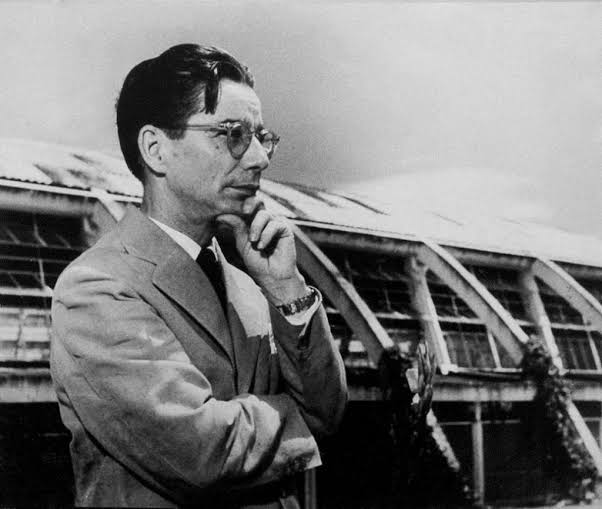
\includegraphics[width=0.7\linewidth]{fig/Anisio-Teixeira}
    \caption{Anísio Teixeira}
    \label{fig:anisio-teixeira}
\end{figure}


Com efeito, tudo fazia crer que Brasília reunia as condições propícias para a
implantação de um sistema de educação modelar. Por um lado, o governo brasileiro
tinha em vista convertê-la “num amplo campo de experimentação de técnicas novas”
(Kubitschek, 2000:140) e, o que é fundamental, assegurava verbas para, com a rapidez
necessária, construir as escolas; por outro lado, na nova Capital havia disponibilidade
plena de espaços físicos para a edificação dos complexos conjuntos escolares propostos,
o que certamente não ocorria nas capitais e grandes cidades já estruturadas.

O plano arquitetônico da cidade, traçado por Lúcio Costa, definira a priori a
estrutura básica da implantação da rede física dos estabelecimentos de ensino (1984:
101), com a distribuição eqüidistante e eqüitativa das escolas. A cidade seria organizada
em super-quadras com blocos residenciais, e nelas se localizariam as escolas primárias,
de modo que as crianças percorressem o menor trajeto possível para atingi-las, sem
interferência com o tráfego de veículos. Já as escolas secundárias, que se destinavam
aos jovens e adolescentes, seriam construídas em locais pré-determinados e de fácil
acesso, onde também se localizariam a igreja, o cinema, o comércio de varejo, etc.

Viñao Frago e Escolano, ao analisarem o surgimento das cidades e o local de
construção da escola, salientam que desde o século XIX, um dos critérios para eleição
do espaço escolar era a segurança das crianças: “Junto à higiene moral e física,
preocupavam também a segurança das crianças - o trânsito de carruagens”(1998:83).

Comentando sobre a circulação das crianças na nova capital, Campos assinala:
\begin{citacao}
    Tendo em vista o sentido das “Unidades de Vizinhança”, pensou o Dr.
    Anísio Teixeira que as escolas seriam distribuídas de tal modo que as
    crianças caminhariam a pé, sem perigo, das respectivas residências para a
    escola ou jardim de infância, e, de retorno dessas unidades escolares às suas
    casas (apartamentos), sem interferência de veículos, cujo tráfego teria vias
    próprias
\end{citacao}

O plano educacional de Brasília, no que tange ao aspecto formal, apresenta
características similares ao planejamento das políticas educacionais que Anísio Teixeira
formulara, anteriormente, para os estados do Rio de Janeiro e da Bahia, e que tiveram
como substrato a projeção de diferentes tipos de construções escolares. Assim, além de
delinear, em linhas gerais, os objetivos e as diretrizes básicas da proposta pedagógica,
detém-se nas especificações relativas aos diferentes prédios e ambientes previstos para
os novos complexos escolares. O pressuposto é que, mediante a descrição detalhada das
características físicas da escola a ser edificada, estariam sendo traduzidos os meios e os
modos pensados para o seu funcionamento, além de que, com a sua construção, ter-se-ia
assegurada a estrutura material para o desenvolvimento da educação, nos moldes
preconizados. Nessa perspectiva, Viñao Frago e Escolano afirmam que:

\begin{citacao}
    Arquitetura escolar é também por si mesma um programa, uma espécie de
    discurso que institui na sua materialidade um sistema de valores, como os de
    ordem, disciplina e vigilância, marcos para a aprendizagem sensorial e
    motora e toda uma semiologia que cobre diferentes símbolos estéticos,
    culturais e também ideológicos (1998:26).
\end{citacao}

Em relação ao conteúdo, o plano apresenta as seguintes características: a) não se
atém ao ensino primário, mas se refere ao sistema educacional como um todo,
abrangendo os diferentes níveis de escolarização, desde o elementar ao superior, numa
perspectiva de continuidade; b) concebe a proposta pedagógica a partir da consideração
de diferentes objetivos e funções atribuídas à escola, em face das mudanças sociais
decorrentes do acelerado desenvolvimento científico e tecnológico, tendo em vista a
formação do novo homem para a vida na sociedade moderna.
É o que diz expressamente a citação abaixo transcrita:
\begin{citacao}
    Como as necessidades da civilização moderna cada vez mais impõem
    obrigações à escola, aumentando-lhe as atribuições e funções, o plano
    consiste – em cada nível de ensino, desde o primário até o superior ou
    terciário, como hoje já se está a chamar – num conjunto de edifícios, com
    funções diversas e considerável variedade de forma e de objetivos, a fim de
    atender a necessidades específicas de ensino e de educação e, além disso, à
    necessidade de vida e convívio social (Teixeira, 1961:195).
    Fica explícito, assim, o propósito de implantar na capital do País um sistema de
    ensino dotado de escolas adequadas à sociedade moderna. É necessário precisar, porém,
    a que sociedade se refere e que tipo de escola seria essa.
\end{citacao}

Descreve \citeaa{Pereira2005} ainda que estruturar um sistema de educação único, democrático,
acessível a todos, independentemente da classe social, centrado no indivíduo e no
desenvolvimento de suas potencialidades e sem a velha dicotomia entre formação geral
e formação especial, entre formação para o trabalho e formação para o lazer, enfim,
entre o útil e o ornamental, que tem caracterizado a educação brasileira ao longo do
tempo. Assim, para transformar um sistema de educação discriminatória, de privilégios,
em um sistema de educação democrático, igualitário, conforme era a pretensão
manifesta de Anísio Teixeira, a instituição escolar teria de ser repensada em seus
fundamentos, alterando seus objetivos, a sua organização e os modos de funcionamento.
Vejamos, a partir do plano educacional, as propostas formuladas, com essa finalidade,
para o sistema de educação da nova Capital.

\subsection{Educação comum e educação especializada}

O forte vínculo da escola com o meio social tem sido, ao longo do tempo, um
dos principais fundamentos de Anísio Teixeira, ao postular a revisão no modelo vigente.
A escola, vista como uma “agência social específica de preparação das crianças para a
sua plena participação na vida social” (Moreira, 197:161), deve permanentemente
adequar-se à sociedade na qual se insere. Educação e sociedade para Anísio não se
desvinculam. Na condição de intelectual liberal, entendia que o papel da escola era ir ao
encontro das “necessidades materiais e espirituais impostas pelo ritmo de
desenvolvimento da sociedade” (Barreira, 1989:33).

Anísio defendia a tese de que a educação deveria assumir prioridade nas
políticas públicas voltadas para o desenvolvimento. Afinal, não era à escola que cabia a
árdua tarefa de preparar a criança para a civilização técnica e industrial, que se
encontrava em permanente mutação?

Essa escola, segundo as suas análises, não seria, obviamente, a que se instituiu
na sociedade agrária, destinada a uma minoria privilegiada – as elites do lazer -, às
quais cabia tão somente aprender e preservar a cultura, enquanto a maioria da população
aprendia diretamente na vida e no próprio trabalho. Nem seria, ainda, a que se
configurou nos primórdios da sociedade industrial, que operava na base de alta
organização e com o operário reduzido à “mão de obra”. A demanda, então, era por uma
escola comum para todos – a escola primária -, para ensinar a ler, escrever e contar,
conhecimentos esses que se tornaram imprescindíveis para o próprio trabalho.

Na percepção de Anísio, a escola, nos tempos atuais, tenderia outra vez a
modificar-se, em função das novas necessidades geradas pela sociedade, que a cada dia
vai-se tornando mais complexa, com novas formas de organização do trabalho
produtivo e de relações sociais. O desenvolvimento tecnológico em curso transforma as
condições de trabalho, mediante o emprego de maquinaria complexa e a decorrente
automação do processo produtivo, provocando mudanças na natureza do trabalho e no
perfil do trabalhador, que deixa de ser “mão-de-obra” para ser “cabeça”, “mente” de
obra (Teixeira, 1976: 365).

Assim, as mudanças da sociedade e do trabalho humano trazem novas
exigências educacionais para a formação do homem comum, já que essa não poderia
limitar-se à mera aquisição dos conhecimentos rudimentares até então previstos para a
escola primária. Para tornar-se capaz de compreender e pensar - e não somente fazer -,
a educação escolar do homem comum teria de ser obrigatoriamente mais longa, com
objetivos mais abrangentes, visando a proporcionar-lhe sólida formação geral e a
aquisição de hábitos e atitudes desejáveis para o trabalho humano e a vida na sociedade
moderna.

O plano educacional de Brasília aponta nessa direção, com referência à
educação comum e obrigatória, destinada a todos, distinguindo-a, porém, da educação
especializada, que se destina a formar os diversos quadros ocupacionais do país
(Teixeira, 1961:197). A formação do cidadão tende, agora, a adquirir uma nova
dimensão e a assumir diferentes finalidades. Em seu artigo intitulado “A educação
comum do homem de hoje” (1976), Anísio Teixeira tece considerações a respeito:

\begin{citacao}
    Cada vez mais precisa o homem, para viver na sociedade artificial e
    complexa, em que se acha inserido, de uma boa educação intelectual, que, à
    falta de outro nome, chamaríamos de geral, seguida ou complementada de
    aprendizagens de natureza ocupacional, destinadas a lhe dar emprego ou
    trabalho. Graças àquela educação geral, a sua posição em relação ao
    trabalho ou emprego se fará muito flexível, habilitando-o a melhorar,
    aperfeiçoar-se e mudar mesmo de setor profissional. Isso quanto à educação
    comum. Quanto à especial, precisamos, como nunca, a equipe dos que irão
    não tanto guardar mas aumentar o conhecimento humano, os pesquisadores;
    depois os organizadores, administradores e diretores – os verdadeiros
    maestros, mestres das grandes orquestrações do trabalho moderno;
    finalmente, em substituição da antiga classe de lazer, preparar os poetas e os
    artistas, isto é, os profissionais destinados a interpretar e dar significação, a
    nos dizer do sentido e do valor da vida e do esforço humano... (Teixeira,
    1976: 364).
\end{citacao}

Essa dupla possibilidade de formação não quer significar, no entanto, o retorno
às antigas discriminações. A educação, concebida para se desenvolver ao longo da vida,
teria um período de escola mais curto ou mais longo, dependendo do indivíduo que, por
sua vontade ou pela sua capacidade, se dispusesse a um patamar ou outro. Assim,
embora se distinguindo mutuamente, a educação geral e educação especial de certa
forma se confundem, formando uma unidade na formação, ou seja: “a educação geral
sendo sempre necessária e a especial correspondendo a um esgalhar-se dessa educação
geral, conforme o nível e o ramo de ocupação a que desejasse o homem se devotar”.


\subsection{Centros de Educação e não ‘apenas’ Escolas }

O sistema de educação proposto para Brasília seria constituído pelos seguintes
tipos de instituições escolares: a) Centros de Educação Elementar, integrado por Jardins
da Infância, Escolas-classe e Escolas-parque; b) Centros de Educação Média, destinados
à Escola Secundária Compreensiva e ao Parque de Educação Média; c) Universidade de
Brasília, composta de Institutos, Faculdades e demais dependências destinadas à
administração, biblioteca, campos de recreação e desportos.
Anísio salienta que “do ponto de vista das construções, o programa constitui um desafio
aos arquitetos de Brasília, oferecendo-lhes a oportunidade para a concepção de novos e
complexos conjuntos escolares”(Idem).O plano educacional foi ajustado às
peculiaridades urbanísticas de Brasília, com a colaboração de Lúcio Costa (Kubitschek,
2000:142). Assim, como a nova Capital é construída em quadras, e cada quadra
abrigaria uma população variável de 2.500 a 3.000 habitantes, a população escolarizável
para os níveis elementar e médio foi calculada segundo essa projeção. Assim: l) para
cada quadra: a) 1 jardim da infância, com 4 salas, para, em 2 turnos de funcionamento,
atender a 160 crianças (8 turmas de 20 crianças); b) 1 escola-classe , com 8 salas, para,
em 2 turnos, atender a 480 alunos (16 turmas de 30 alunos); e, 2) para cada grupo de 4
quadras: a) 1 escola-parque, destinada a atender, em 2 turnos, a cerca de 2.000 alunos de
4 escolas-classe, em atividades de iniciação para o trabalho (para alunos de 7 a 14 anos),
nas pequenas oficinas de artes industriais (tecelagem, tapeçaria, encadernação,
cerâmica, cartonagem, bordado e trabalhos em couro, lã, madeira, metal, etc.), além da
participação dirigida dos alunos de 7 a 14 anos em atividades artísticas, sociais e de
recreação (música, dança, teatro, pintura, exposições, grêmios, educação física). Além
dos pavilhões e salas-ambiente para o desenvolvimento dessas atividades, constava
ainda a construção de dependências para refeitório e administração, além de pequenos
conjuntos residenciais, para jovens de 7 a 14 anos, sem família, sujeitos às mesmas
atividades que os alunos externos.

No que tange ao nível médio, a previsão era de um Centro de Educação Média
para cada grupo populacional de 45.000 habitantes (Idem, p.143). Cada Centro seria
constituído de um conjunto de edifícios, para abrigar cerca de 2.250 alunos de 11 a 18
anos, de forma a adequar-se ao exercício das atividades programadas. Assim, a
arquitetura escolar previa: centro cultural, teatro e exposições; biblioteca e museus;
centro de serviços gerais; escola média compreensiva, incluindo ginásio, colégio, escola
comercial, técnico-industrial, curso normal ou pedagógico e escola agrícola; centro de
educação física e esportes em geral.

Dada a abrangência do programa, é utilizado o termo Centro no lugar de Escola.
\begin{citacao}
    Já não se trata de escolas e salas de aula, mas de todo um conjunto de locais,
    em que as crianças se distribuem, entregues às atividades de ‘estudo’, de
    ‘trabalho’, de ‘recreação’, de ‘reunião’, de ‘administração’, de ‘decisão’ e de
    vida e de convívio no mais amplo sentido desse termo. A arquitetura escolar
    deve assim combinar aspectos da ‘escola tradicional’ com os da ‘oficina’,
    do ‘clube’ de esportes e de recreio, da ‘casa’, do ‘comércio’, do
    ‘restaurante’, do ‘teatro’, compreendendo, talvez, o programa mais
    complexo e mais diversificado de todas as arquiteturas especiais (Teixeira,
    1961:197).
\end{citacao}

É tal a amplitude e a complexidade do Centro de Educação Elementar que
Anísio o compara a uma Universidade Infantil (Idem, p.195). Essa grandeza também se
reproduz no Centro de Educação Média, que passa a ter a responsabilidade por um
programa consideravelmente diversificado. Ao justificar a criação de “centros”, Anísio
pondera que nos diferentes níveis de ensino as instituições devem ser
\begin{citacao}
    organizadas tendo em vista constituírem-se verdadeiras comunidades, com
    as suas diversas funções e considerável variedade de atividades, a serem
    distribuídas por um conjunto de edifícios e locais a lembrar, tanto no nível
    primário, como no secundário ou no superior, verdadeiros conjuntos
    universitários (Teixeira, 1962:27).
\end{citacao}

\subsection{Educação primária integral}

No plano educacional de Brasília é retomada a idéia de Escola-Parque e das
Escolas-Classe, que constituíram o cerne da política educacional proposta e executada
por Anísio Teixeira, na Bahia, e que se materializou como a criação do Centro
Educacional Carneiro Ribeiro, em Salvador, concebido com o primeiro centro de
demonstração do ensino primário no País. A iniciativa, que, segundo as palavras do
grande educador, foi “uma tentativa de se produzir um modelo para a nossa escola
primária” (Teixeira, 1967:247), agora, seria adotada na nova Capital. Diferentemente
daquela experiência pioneira de educação primária, que, nos 50, fora implantada numa
das chamadas “invasões”, onde morava uma população em situação de extrema
pobreza, percorridos dez anos, experiência similar seria instalada no centro
administrativo e político do País, destinada a todas as classes sociais, “de forma a
permitir que um filho de ministro de Estado estudasse, lado a lado, de um filho de
operário” (Kubitschek, 1000:141).

A escolarização seria iniciada no Jardim de Infância, para crianças de 4 a 6 anos
de idade e, em seguida, os alunos ingressariam na Escola-Classe, concebida para a
educação intelectual sistemática de alunos de 7 a 14 anos, complementando,
paralelamente, a sua formação na Escola-Parque, com vistas ao desenvolvimento
artístico, físico e recreativo e sua iniciação para o trabalho. A idéia básica nessa
concepção, segundo explicita o plano, é “juntar o ensino propriamente intencional, da
sala de aula, com a auto-educação resultante de atividades de que os alunos participem
com plena responsabilidade” (Teixeira, 1961:197). Nessas condições,
\begin{citacao}
    a criança, além das quatro horas de educação convencional, no edifício da
    escola-classe, onde aprende a estudar, conta com outras quatro horas de
    atividades de trabalho, de educação física e de educação social, atividades
    em que se empenha individualmente ou em grupo, aprendendo, portanto, a
    trabalhar e a conviver (Idem).
\end{citacao}

Configura-se, assim, a idéia de uma educação integral, que se volta para o
indivíduo em todas as suas dimensões. A escola completa, rica, variada, formativa por
excelência e integrada ao espaço vivificante do mundo, possibilitaria aos alunos
participação em experiências educativas diversificadas, pelas quais se habilitariam para
a ação inteligente em sua vida. Para isso a jornada escolar se estenderia,
necessariamente, para oito horas diárias, “tempo para se fazer uma escola de formação
de hábitos de vida, de comportamento, de trabalho e de julgamento moral e intelectual”
(Teixeira, 1957:4).

A sua organização far-se-ia em termos de escola-comunidade, mediante um
currículo de aprendizagem por participação, o que transformaria a escola em local de
vida e de atividades adequadas às idades. Para Anísio, a filosofia da escola consistia em
“oferecer à criança um retrato da vida em sociedade, com as suas atividades
diversificadas e seu ritmo de ‘preparação’ e ‘execução’, dando-lhe as experiências de
estudo e de ação responsáveis” (Teixeira, 1962:25). Numa sociedade como a brasileira,
marcada pelo subdesenvolvimento e intensa estratificação social, a escola não poderia
mais ser uma instituição simples, e a escola primária era a instituição que, no seu ponto
de vista, deveria promover a igualdade de oportunidades, essência do regime
democrático.

\subsection{Ensino médio: preparação para o trabalho e continuidade dos estudos}
A idéia presente na organização do ensino médio é a de reunir, num único
Centro, todos os cursos de grau médio, permitindo maior sociabilidade aos jovens, que,
embora freqüentando classes diferentes, tivessem, em comum, atividades na biblioteca,
na piscina, nos campos de esporte, nos grêmios, no refeitório, etc. Nesse sentido, o
plano educacional de Brasília previa a construção de seis blocos construtivos agrupados
em torno de uma praça central. (Teixeira, 1961:198).

O Centro de Ensino Médio destinava-se a oferecer a cada adolescente a real
oportunidade para cultivar o seu talento, tendo em vista dupla finalidade: preparar-se
diretamente para o trabalho ou prosseguir a sua educação no nível superior (Idem, p.
195). Tratava-se, assim, de reconfigurar o ensino secundário, de caráter enciclopédico e
‘supostamente’ propedêutico ao ensino superior, que, na opinião de Anísio, falhava
inclusive na finalidade de cultura geral, em face da uniformidade, do aligeiramento e da
fragmentação, afora a prática de métodos obsoletos de memorização, a imposição de
conhecimentos inertes e o formalismo das notas e dos exames. Numa nação moderna,
em que o curso secundário não se destina a poucos, mas a todos os jovens, impunha-se
modificar sua finalidade e objetivos (Teixeira, 1958:1).

No lugar do ensino uniforme, a perspectiva de Anísio era adaptar a escola aos
tipos de inteligência e aptidão dos alunos, tendo em vista atender as diferenças
individuais. Basicamente, propunha três modalidades de estudos: a) curso geral prático,
comum, para todos ou para a grande maioria, visava a ministrar cultura geral, com
ênfase na língua vernácula e literatura brasileira, nas matemáticas e nas ciências físicas
e sociais aplicadas; b) cursos enriquecidos com línguas estrangeiras e estudos teóricos,
como desdobramento do primeiro, para aqueles que se mostrassem interessados ou
capazes de estudos dessa natureza; e, c) cursos técnicos para os inclinados à
especialização tecnológica. Os exames vestibulares, aberto a todos os alunos, visariam a
apurar antes a capacidade intelectual do que a erudição para o ensino superior (Idem: 2).

A nova concepção do ensino médio apontava para uma educação extensiva, de
dedicação exclusiva. Nesses termos,

\begin{citacao}
    Todos os estudos, de verdadeira e autêntica formação para o trabalho, seja o
    trabalho intelectual, científico, técnico, artístico ou material, dificilmente
    podem ser estudados em tempo parcial, dificilmente podem ser feitos em
    períodos apenas de aula, exigindo além disso e, sempre, longos períodos de
    estudo individual – e para tal grandes bibliotecas, com abundância de livros
    e de espaço para o estudante – longos períodos de prática em laboratórios,
    salas-ambiente, ateliês, etc., e longos períodos de convivência entre os que
    estão formando e os professores. Somente com professores de tempo
    integral e alunos de tempo integral poderemos formar esses trabalhadores de
    nível médio (...) (Teixeira, 1957:17).
\end{citacao}

O processo de diversificação de funções e ocupações da sociedade moderna
industrial estar-se-ia constituindo em fator determinante para a proposta de uma
educação mais prolongada e mais variada. Daí a necessidade de reorientação da escola
no sentido de torná-la uma escola de trabalho e de preparo real, afirma \citeaa{Pereira2005}.

Sob certo sentido, observamos que o Distrito Federal deveria ser referência no ENEM, e até é, de os microdados do ENEM da página do \citeaa{INEP2019} com ferramentas de Data Science notamos que Brasília é a 5º melhor estado no critério da nota normalizada combinada de português, matemática e redação.


% Please add the following required packages to your document preamble:
% \usepackage[table,xcdraw]{xcolor}
% If you use beamer only pass "xcolor=table" option, i.e. \documentclass[xcolor=table]{beamer}
% \usepackage[normalem]{ulem}
% \useunder{\uline}{\ul}{}
\begin{table}[]
    \centering
    \resizebox{1\textwidth}{!}{
        \begin{tabular}{llrrrrrrrrr}
            &
            &
            &
            \multicolumn{2}{c}{\cellcolor[HTML]{4F81BD}{\color[HTML]{FFFFFF} Matemática}} &
            \multicolumn{2}{c}{\cellcolor[HTML]{4F81BD}{\color[HTML]{FFFFFF} Português}} &
            \multicolumn{2}{c}{\cellcolor[HTML]{4F81BD}{\color[HTML]{FFFFFF} Redação}} &
            \multicolumn{2}{c}{\cellcolor[HTML]{4F81BD}{\color[HTML]{FFFFFF} Geral}} \\
            \rowcolor[HTML]{4F81BD}
            \multicolumn{1}{c}{\cellcolor[HTML]{4F81BD}{\color[HTML]{FFFFFF} UF}} &
            \multicolumn{1}{c}{\cellcolor[HTML]{4F81BD}{\color[HTML]{FFFFFF} Nome}} &
            \multicolumn{1}{c}{\cellcolor[HTML]{4F81BD}{\color[HTML]{FFFFFF} n}} &
            \multicolumn{1}{c}{\cellcolor[HTML]{4F81BD}{\color[HTML]{FFFFFF} média ($\mu$)}} &
            \multicolumn{1}{c}{\cellcolor[HTML]{4F81BD}{\color[HTML]{FFFFFF} desvio ($\sigma$)}} &
            \multicolumn{1}{c}{\cellcolor[HTML]{4F81BD}{\color[HTML]{FFFFFF} média ($\mu$)}} &
            \multicolumn{1}{c}{\cellcolor[HTML]{4F81BD}{\color[HTML]{FFFFFF} desvio ($\sigma$)}} &
            \multicolumn{1}{c}{\cellcolor[HTML]{4F81BD}{\color[HTML]{FFFFFF} média ($\mu$)}} &
            \multicolumn{1}{c}{\cellcolor[HTML]{4F81BD}{\color[HTML]{FFFFFF} desvio ($\sigma$)}} &
            \multicolumn{1}{c}{\cellcolor[HTML]{4F81BD}{\color[HTML]{FFFFFF} média ($\mu$)}} &
            \multicolumn{1}{c}{\cellcolor[HTML]{4F81BD}{\color[HTML]{FFFFFF} desvio ($\sigma$)}} \\

            33 & Rio de Janeiro      & 821.192   & 5,48 & 1,11 & 6,66 & 0,85 & 5,43 & 1,89 & 5,85 & 1,07 \\
            \rowcolor[HTML]{DCE6F1}
            35 & São Paulo           & 2.067.998 & 5,52 & 1,09 & 6,70 & 0,84 & 5,32 & 1,75 & 5,84 & 1,03 \\
            31 & Minas Gerais        & 1.318.779 & 5,50 & 1,11 & 6,60 & 0,85 & 5,42 & 1,87 & 5,83 & 1,08 \\
            \rowcolor[HTML]{DCE6F1}
            42 & Santa Catarina      & 251.020   & 5,53 & 1,06 & 6,65 & 0,81 & 5,29 & 1,72 & 5,82 & 0,99 \\
            53 & Distrito Federal    & 227.700   & 5,39 & 1,12 & 6,64 & 0,90 & 5,33 & 1,82 & 5,78 & 1,08 \\
            \rowcolor[HTML]{DCE6F1}
            43 & Rio Grande do Sul   & 538.528   & 5,43 & 1,03 & 6,64 & 0,82 & 5,28 & 1,77 & 5,78 & 1,00 \\
            41 & Paraná              & 523.804   & 5,44 & 1,06 & 6,62 & 0,83 & 5,18 & 1,72 & 5,74 & 1,00 \\
            \rowcolor[HTML]{DCE6F1}
            32 & Espírito Santo      & 249.704   & 5,44 & 1,09 & 6,53 & 0,84 & 5,27 & 1,89 & 5,74 & 1,07 \\
            52 & Goiás               & 411.025   & 5,28 & 1,04 & 6,44 & 0,87 & 5,21 & 1,90 & 5,64 & 1,08 \\
            \rowcolor[HTML]{DCE6F1}
            24 & Rio Grande do Norte & 283.115   & 5,23 & 1,02 & 6,38 & 0,87 & 5,11 & 1,85 & 5,57 & 1,04 \\
            23 & Ceará               & 695.751   & 5,23 & 1,04 & 6,34 & 0,88 & 5,13 & 2,01 & 5,56 & 1,11 \\
            \rowcolor[HTML]{DCE6F1}
            28 & Sergipe             & 164.904   & 5,13 & 1,00 & 6,30 & 0,87 & 5,21 & 1,94 & 5,54 & 1,06 \\
            50 & Mato Grosso do Sul  & 164.517   & 5,22 & 1,01 & 6,41 & 0,86 & 4,99 & 1,86 & 5,53 & 1,04 \\
            \rowcolor[HTML]{DCE6F1}
            26 & Pernambuco          & 671.737   & 5,21 & 1,01 & 6,34 & 0,86 & 5,01 & 1,95 & 5,51 & 1,06 \\
            25 & Paraíba             & 341.925   & 5,16 & 1,00 & 6,31 & 0,85 & 5,08 & 1,91 & 5,51 & 1,04 \\
            \rowcolor[HTML]{DCE6F1}
            29 & Bahia               & 894.796   & 5,09 & 0,97 & 6,30 & 0,87 & 5,08 & 1,86 & 5,49 & 1,02 \\
            22 & Piauí               & 265.903   & 5,06 & 0,99 & 6,19 & 0,88 & 4,99 & 1,93 & 5,41 & 1,06 \\
            \rowcolor[HTML]{DCE6F1}
            27 & Alagoas             & 210.719   & 5,05 & 0,96 & 6,20 & 0,85 & 4,97 & 1,94 & 5,40 & 1,03 \\
            51 & Mato Grosso         & 223.016   & 5,12 & 0,97 & 6,29 & 0,85 & 4,80 & 1,93 & 5,39 & 1,05 \\
            \rowcolor[HTML]{DCE6F1}
            15 & Pará                & 640.706   & 4,98 & 0,89 & 6,19 & 0,84 & 4,96 & 1,91 & 5,37 & 0,99 \\
            17 & Tocantins           & 123.542   & 5,02 & 0,92 & 6,16 & 0,90 & 4,84 & 1,84 & 5,33 & 1,02 \\
            \rowcolor[HTML]{DCE6F1}
            11 & Rondônia            & 142.699   & 5,03 & 0,89 & 6,23 & 0,82 & 4,71 & 1,80 & 5,32 & 0,95 \\
            14 & Roraima             & 34.244    & 5,05 & 0,93 & 6,25 & 0,86 & 4,68 & 1,91 & 5,32 & 1,02 \\
            \rowcolor[HTML]{DCE6F1}
            21 & Maranhão            & 506.433   & 4,94 & 0,87 & 6,14 & 0,85 & 4,78 & 1,89 & 5,28 & 0,99 \\
            16 & Amapá               & 90.961    & 4,91 & 0,83 & 6,16 & 0,84 & 4,77 & 1,83 & 5,28 & 0,95 \\
            \rowcolor[HTML]{DCE6F1}
            13 & Amazonas            & 288.926   & 4,95 & 0,86 & 6,18 & 0,85 & 4,69 & 1,82 & 5,27 & 0,97 \\
            12 & Acre                & 91.444    & 4,91 & 0,84 & 6,16 & 0,84 & 4,72 & 1,85 & 5,26 & 0,96
        \end{tabular}
    }
    \caption{ Desempenho ENEM 2017/2018 por UF do aluno - Notas normalizadas 0 a 10 - ordenado por média ($\mu$) geral}
    \label{table:ENEM}
\end{table}
